\documentclass{ieeeaccess}
\usepackage{cite}
\usepackage{amsmath,amssymb}
\usepackage{graphicx}
\usepackage{booktabs}
\usepackage{url}
\begin{document}
\history{Draft manuscript: 22 November 2026. Not submitted.}
\doi{DRAFT --- no DOI assigned}
\vol{DRAFT}
\year{2026}
% DRAFT: replace author, email, biography, and approval details before submission.
\title{Does a Truthful Model-Selected Cue Increase Bounded Feature-Space Evasion of Phishing Detectors? A Matched-Control Study}
\author{\uppercase{Author name to confirm}\authorrefmark{1}}
\address[1]{Informatics Institute of Technology, Sri Lanka, affiliated with the University of Westminster, London, U.K.}
\markboth{Author et al.: Truthful Model-Selected Cues and Phishing Detector Evasion}{Author et al.: Truthful Model-Selected Cues and Phishing Detector Evasion}
\begin{abstract}
The disclosure of a phishing detector's factual, model-selected cue may help a recipient understand a decision, but the same cue may also guide an adversary. We estimate the incremental effect of cue selection by comparing it with a truthful fact selected independently of model relevance from the same preassigned feature family. Two detectors were trained on 9,214 group-split CompPhish v4 examples and evaluated on a frozen final partition of 2,303 examples. The primary endpoint was a binary prediction flip after an abstract, train-bounded feature-vector change, with one coordinate change and at most five binary queries including the initial verdict. On initially detected phishing examples eligible for distinct same-family cues, model-selected and independently selected cues produced bypass rates of 77.03\% and 23.84\% for logistic regression (344 pairs; paired difference 53.20 percentage points), and 73.91\% and 60.20\% for shallow gradient boosting (299 pairs; difference 13.71 points). Connected-group bootstrap intervals with 97.5\% coverage were 45.79--60.56 and 8.87--18.75 points, respectively. These positive contrasts quantify a coordinate-priority advantage in the implemented search. The changed vectors were not demonstrated to correspond to valid websites or URLs. Coverage of the matched population and dataset source confounding further limit generalization. The study provides a reproducible, narrow disclosure comparison rather than evidence of operational phishing-page evasion.
\end{abstract}
\begin{keywords}
adversarial machine learning, explanation disclosure, feature-space evasion, phishing detection, reproducibility
\end{keywords}
\titlepgskip=-21pt
\maketitle

\section{Introduction}
\PARstart{P}{hishing} detectors increasingly use machine-learned representations of URLs and page content. A factual reason for a positive verdict can be useful to a recipient, yet it can also identify where a bounded adversary should search for a prediction flip. Prior work already establishes feature-guided attacks and the distinction between changing model inputs and changing a functioning phishing page \cite{figa,spacephish,multispacephish}. The question here is narrower: conditional on disclosing one truthful fact, how much additional search advantage arises from selecting that fact for its local relevance to the detector?

We compare three arms: verdict only (V), a same-family truthful fact selected without relevance information (S), and a distinct truthful fact selected for local model relevance in that family (M-family). In each arm the simulated search has the same candidate values, initial vector, binary verdict interface, and query and coordinate budgets. The primary estimand is the within-start difference in observed bypass between M-family and S among starts eligible for both. This matched design isolates cue identity more closely than an M-versus-V comparison, although it does not isolate every possible feature-priority mechanism.

The contribution is an auditable comparison on two frozen detectors with connected-group uncertainty intervals, source-derived feature checks, and explicit denominator accounting. The result concerns abstract model-input vectors. It does not measure recipient comprehension, deployed explanations, or feasible edits to phishing pages.

\section{Related Work}
Feature Importance Guided Attack (FIGA) studies feature-importance-guided tabular evasion and separately evaluates phishing problem-space transformations \cite{figa}. SpacePhish formalizes the threat model and different evasion spaces for phishing detectors \cite{spacephish}; Multi-SpacePhish extends evaluation across multiple spaces and settings \cite{multispacephish}. Work on gray-box phishing attacks varies attacker feature knowledge \cite{lnuphish}, while post-hoc explanation studies show that explanation information can guide black-box attacks in other contexts \cite{quan}. These works preclude a claim that feature guidance or explanation risk itself is new. Our empirical distinction is a factual model-selected cue compared with an independently chosen factual cue from the same feature family under a shared search. The current work does not establish priority over all previous matched-disclosure studies.

\section{Data and Experimental Design}
\subsection{Dataset, grouping, and features}
CompPhish v4 supplies 15,358 labeled URL/HTML pairs and associated feature material \cite{compphishdata,compphishpaper}. We excluded three exact URL--HTML--label duplicate rows from the primary analysis, leaving 15,355. Connected domain/template group IDs were assigned atomically to 60\% training (9,214), 15\% development (2,303), 10\% method validation (1,535), and 15\% final (2,303). The final partition contains 1,080 phishing and 1,223 legitimate rows. Distinct URL/page pairs sharing HTML were retained, including mixed-label exact-HTML groups. Group IDs are a leakage-control proxy, not proof of independence.

Twelve registered URL and HTML features were recomputed from archived source material; row identifiers, URL text, hashes, labels, and split metadata were excluded from model inputs. Three published HTML feature columns disagreed with the archived HTML on sampled rows, so source-derived values were used consistently. A malformed HTML record required documented numeric-entity recovery. The independent final audit compared all 27,636 feature values across 2,303 final rows with zero mismatches against the frozen source-derived matrix. Archived HTML was handled as inert local data; no live URLs were visited.

The registered families are URL structure (length, path slash count, query parameter count, HTTPS use), URL lexical (numeric proportion, hostname digit ratio, entropy, embedded URL flag), HTML structure (form and image counts, inline event handlers), and HTML content (missing title). The last family has only one registered feature and cannot supply two distinct cues. The release's phishing and legitimate samples have different acquisition sources, and row-level timestamps are unavailable. Therefore, held-out metrics are within-dataset measurements rather than evidence of source- or time-independent detection.

\subsection{Detectors and operating point}
We fitted L2 logistic regression with train-only standardization and a shallow gradient-boosted tree model on the same 9,214 training records. Small, fixed hyperparameter grids were selected by development average precision. A planned 1\% empirical development false-positive-rate (FPR) target gave logistic recall 38.43\%, below the prespecified 50\% feasibility floor. Before method validation or final evaluation, protocol v2 changed the common target to 2\%, the smallest audited target at which both frozen model families passed that floor. The 2\% development point yielded recalls of 54.81\% (logistic) and 70.56\% (boosting), each with 24/1,223 development benign false positives. The selected logistic penalty parameter was $C=10$; the selected boosted model used depth 3 and 200 estimators. The amended frozen score thresholds were 0.7911127721 and 0.7929628727, respectively, with a positive decision for scores at or above the threshold. No model was refitted on development. This is a development-informed amendment, not a preplanned 2\% threshold or a population FPR guarantee.

\begin{table*}[t]
\centering\caption{Frozen final matched-start results. All three bypass rates in a detector row share the same eligible starts. Intervals cover the paired difference using connected-group resampling and Bonferroni adjustment.}
\label{tab:primary}
\begin{tabular}{lrrrrrrr}
\toprule
Detector & Rows & Groups & V (\%) & S (\%) & M-family (\%) & $M-S$ (points) & 97.5\% interval (points) \\
\midrule
Logistic regression & 344 & 268 & 43.60 & 23.84 & 77.03 & 53.20 & [45.79, 60.56] \\
Gradient boosting & 299 & 237 & 66.89 & 60.20 & 73.91 & 13.71 & [8.87, 18.75] \\
\bottomrule
\end{tabular}
\end{table*}
\begin{figure*}[t]
\centering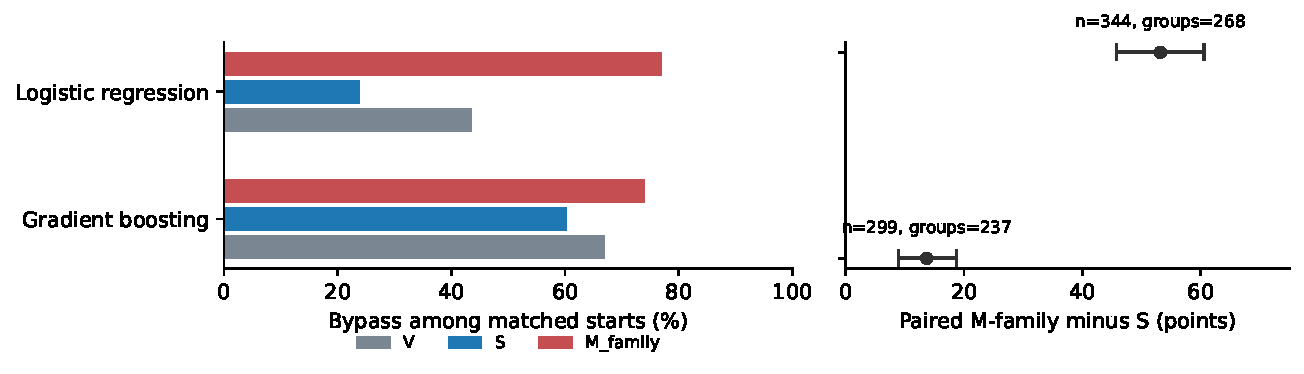
\includegraphics[width=0.88\textwidth]{figures/frozen_matched_results.pdf}
\caption{Frozen matched-start bypass rates and paired M-family minus S contrasts. Error bars show 97.5\% connected-group bootstrap intervals adjusted across the two detector contrasts.}
\label{fig:primary}
\end{figure*}

\subsection{Disclosure and abstract search}
For each initially detected phishing start, a feature family was preassigned by a seeded hash of its row serial number. S used the first available factual feature in that family without using model relevance. M-family used a different eligible feature in the same family with the largest positive local score reduction when replaced by its train-only median or mode. The evaluator used the score only to select the factual cue; the simulated attacker received no score, gradient, coefficient, or threshold. A family with only one registered feature could not yield a distinct matched pair. Eligibility was determined before arm outcomes.

Candidate numeric coordinates used train-derived 5th and 95th percentiles, rounded inward for integer features; binary coordinates toggled. Each candidate started from the original vector. A fixed search tried one-coordinate candidates before larger combinations, ranking the disclosed coordinate first in S and M-family and using registry order in V. It counted the initial verdict and every submitted candidate as binary queries, stopping at the first negative prediction or budget exhaustion. The development pooled-success rule selected one changed coordinate and five total queries, without selecting on the arm contrast. K0 (anonymous coordinate interface) was the only confirmatory knowledge condition. K2 was operationally identical because this search did not consume semantic feature definitions; a knowledge interaction was not tested.

All three arms shared the same candidate grammar and query cap. This grammar does not enforce all dependencies among URL and HTML features. An edited vector may fail to correspond to any valid or visible page. Consequently, ``bypass'' throughout means a model prediction flip under this abstract search.

\subsection{Frozen analysis}
Let $Y_{ia}\in\{0,1\}$ indicate whether arm $a$ obtained a flip for matched start $i$ within budget. The primary paired contrast for each detector was
\begin{equation}
\widehat{\Delta}=\frac{1}{N}\sum_{i=1}^{N}(Y_{iM}-Y_{iS}).
\end{equation}
The analysis used all initially detected phishing starts with both a factual S and a distinct eligible same-family M cue. It resampled connected groups 10,000 times with replacement, retained their paired rows, and computed percentile intervals with 97.5\% coverage for two detector contrasts (Bonferroni familywise 5\%). The frozen protocol also defined a $\pm5$-point equivalence margin; the positive final intervals do not require an equivalence interpretation. A method-validation partition checked the frozen implementation and factual recomputation without retuning. A hash manifest then fixed ten input and analysis artifacts before the final split was evaluated once.




\section{Frozen Final Results}
\subsection{Detector context}
At the frozen thresholds, logistic regression had 26/1,223 benign false positives (2.13\% FPR), detected 589/1,080 phishing rows (54.54\% recall), and achieved 95.77\% precision, 0.9212 receiver-operating-characteristic area, and 0.9226 average precision. Boosting had 27/1,223 benign false positives (2.21\% FPR), detected 759/1,080 phishing rows (70.28\% recall), and achieved 96.56\% precision, 0.9608 receiver-operating-characteristic area, and 0.9586 average precision. Both final empirical FPRs slightly exceed the 2\% development target. Their Wilson 95\% FPR intervals are 1.45--3.10\% and 1.52--3.19\%, respectively.



\subsection{Matched cue contrast and coverage}
Table~\ref{tab:primary} and Fig.~\ref{fig:primary} give the primary results. Logistic regression had 193 M-only versus 10 S-only bypasses; boosting had 43 versus 2. Both adjusted intervals exclude zero. Mean binary queries on matched starts were 2.80 for M-family and 4.43 for S under logistic regression, and 3.49 and 3.82 under boosting. These are descriptive costs under early stopping, not a separately adjusted hypothesis test.



Only 344/589 (58.4\%) initially detected logistic starts and 299/759 (39.4\%) boosted starts entered the distinct same-family comparison. Across \emph{all} initially detected starts, V/S/M-global-with-V-fallback bypass rates were 49.1/27.5/92.7\% for logistic regression and 68.4/62.5/74.6\% for boosting. Those policy-level rates have different denominators and an unrestricted global M cue; they are not estimates of the primary paired contrast. A sensitivity check at one changed coordinate and 40 total queries found identical V, S, and M-family rates within each detector: 98.84\% for logistic regression and 89.97\% for boosting. Thus the measured cue-priority advantage at five queries disappears under this expanded one-coordinate query cap. The full coordinate/query-budget grid is preserved in the final aggregate result manifest.

\section{Discussion and Limitations}
The positive paired differences show that the implemented model-selected cue placed more successful coordinates earlier in this bounded feature-vector search than the same-family independently chosen fact. The size of that advantage depended strongly on detector family and eligible population. Because the search ranks a disclosed coordinate first, the measured effect is specifically a coordinate-priority effect under this algorithm, not a universal effect of any truthful explanation.

The most consequential limitation is feasibility: feature dependencies were not fully enforced and no altered vector was mapped to a functioning URL or HTML page. These results cannot support claims of deployable phishing evasion, real-page modification, or user harm from a live explanation. Other limitations include one class-source-confounded dataset; unavailable row timestamps; two detector families; provisional connected groups; selected-feature disagreements with the published table; and reduced same-family matched coverage, especially for boosting. The frozen attack log recorded changed-coordinate count and binary-query cost but did not record normalized perturbation magnitude, despite its mention in the earlier protocol. A magnitude distribution therefore cannot be reported. The K0/K2 knowledge interaction and the proposed conditional minimax selector were not tested. No human study evaluated explanation usefulness or comprehension.

The student reported supervisor acceptance of a Class 1 declaration for this PoC and local dataset processing; the approval artifact was not independently inspected in this research record. Before external submission, authors should verify the institutional record and describe its approved scope accurately. The experiment used archived data offline and no human participants or live page requests.

\section{Reproducibility and Conclusion}
The repository contains the versioned feature registry, group/split manifest, source-derived matrix manifest, model protocol and thresholds, attack implementation, method-validation output, final-freeze hashes, final aggregate JSON, and a read-only HTML results demo. Raw archive files and row-level logs remain local and are not redistributed. The final evaluation was run once after hash verification; its aggregate artifact records the freeze-manifest and selected-log SHA-256 values. Reproduction requires the licensed CompPhish v4 archive and the pinned parser/modeling dependencies.

Under a one-coordinate, five-query abstract feature-vector budget, a truthful model-selected cue increased observed bypass relative to a distinct truthful fact from the same feature family in both frozen detectors. The conclusion is limited to eligible matched starts and this offline search. A next study should enforce page-space dependencies, document perturbation magnitude, test additional datasets and detector families, and examine whether recipients gain a measurable benefit from the cues.

\section*{Acknowledgment and AI disclosure}
OpenAI Codex assisted in drafting prose and LaTeX, generating the figure code, and checking numerical statements against frozen repository manifests. The author is responsible for verifying all text, references, and results before submission. No funding statement is supplied in this draft.

\begin{thebibliography}{00}
\bibitem{compphishdata} R. Goenka, ``CompPhish,'' Mendeley Data, ver. 4, 2026, doi: 10.17632/fmbs4kp9wz.4.
\bibitem{compphishpaper} R. Goenka \emph{et al.}, ``CompPhish: A comprehensive dataset for diversified phishing detection,'' \emph{Data in Brief}, 2026, doi: 10.1016/j.dib.2026.113219.
\bibitem{figa} G. Gressel \emph{et al.}, ``Feature Importance Guided Attack: A Model Agnostic Adversarial Attack,'' arXiv:2106.14815, 2021, revised 2023.
\bibitem{spacephish} G. Apruzzese \emph{et al.}, ``SpacePhish: The Evasion-space of Adversarial Attacks against Phishing Website Detectors using Machine Learning,'' in \emph{Proc. ACSAC}, 2022, doi: 10.1145/3564625.3567980.
\bibitem{multispacephish} Y. Yuan \emph{et al.}, ``Multi-SpacePhish: Extending the Evasion-space of Adversarial Attacks against Phishing Website Detectors Using Machine Learning,'' \emph{Digital Threats: Research and Practice}, 2024, doi: 10.1145/3638253.
\bibitem{lnuphish} G. Apruzzese and V. S. Subrahmanian, ``Mitigating Adversarial Gray-Box Attacks Against Phishing Detectors,'' \emph{IEEE Trans. Dependable Secure Comput.}, doi: 10.1109/TDSC.2022.3210029.
\bibitem{quan} P. Quan \emph{et al.}, ``On the amplification of security and privacy risks by post-hoc explanations in machine learning models,'' arXiv:2206.14004, 2022.
\end{thebibliography}

\begin{IEEEbiographynophoto}{Author name to confirm}
The author's verified full name, degree information, and short biography will be added before submission.
\end{IEEEbiographynophoto}
\EOD
\end{document}
